\documentclass[11pt,twoside,a4paper]{article}
% http://www-h.eng.cam.ac.uk/help/tpl/textprocessing/latex_maths+pix/node6.html symboles de math
% http://fr.wikibooks.org/wiki/Programmation_LaTeX Programmation latex (wikibook)
%=========================== En-Tete =================================
%--- Insertion de paquetages (optionnel) ---
\usepackage[french]{babel}   % pour dire que le texte est en fran{\'e}ais
\usepackage{a4}	             % pour la taille   
\usepackage[T1]{fontenc}     % pour les font postscript
\usepackage{epsfig}          % pour gerer les images
%\usepackage{psfig}
\usepackage{amsmath, amsthm} % tres bon mode mathematique
\usepackage{amsfonts,amssymb}% permet la definition des ensembles
\usepackage{float}           % pour le placement des figure
\usepackage{verbatim}

\usepackage{longtable} % pour les tableaux de plusieurs pages

\usepackage[table]{xcolor} % couleur de fond des cellules de tableaux

\usepackage{lastpage}

\usepackage{multirow}

\usepackage{multicol} % pour {\'e}crire dans certaines zones en colonnes : \begin{multicols}{nb colonnes}...\end{multicols} 

% \usepackage[top=1.5cm, bottom=1.5cm, left=1.5cm, right=1.5cm]{geometry}
% gauche, haut, droite, bas, entete, ente2txt, pied, txt2pied
\usepackage{vmargin}
\setmarginsrb{1.00cm}{1.00cm}{1.00cm}{1.00cm}{15pt}{3pt}{15pt}{3pt}

\usepackage{lscape} % changement orientation page
%\usepackage{frbib} % enlever pour obtenir references en anglais
% --- style de page (pour les en-tete) ---
\pagestyle{empty}

% % % en-tete et pieds de page configurables : fancyhdr.sty

% http://www.trustonme.net/didactels/250.html

% http://ww3.ac-poitiers.fr/math/tex/pratique/entete/entete.htm
% http://www.ctan.org/tex-archive/macros/latex/contrib/fancyhdr/fancyhdr.pdf
% \usepackage{fancyhdr}
% \pagestyle{fancy}
% % \newcommand{\chaptermark}[1]{\markboth{#1}{}}
% % \newcommand{\sectionmark}[1]{\markright{\thesection\ #1}}
% \fancyhf{}
% \fancyhead[LE,RO]{\bfseries\thepage}
% \fancyhead[LO]{\bfseries\rightmark}
% \fancyhead[RE]{\bfseries\leftmark}
% \fancyfoot[LE]{\thepage /\pageref{LastPage} \hfill
	% TITLE
% \hfill 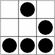
\includegraphics[width=0.5cm]{img/logo_glider.png} }
% \fancyfoot[RO]{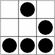
\includegraphics[width=0.5cm]{img/logo_glider.png} \hfill
	% TITLE
% \hfill \thepage /\pageref{LastPage}}
% \renewcommand{\headrulewidth}{0.5pt}
% \renewcommand{\footrulewidth}{0.5pt}
% \addtolength{\headheight}{0.5pt}
% \fancypagestyle{plain}{
	% \fancyhead{}
	% \renewcommand{\headrulewidth}{0pt}
% }


%============================= Corps =================================
\begin{document}

\setlength\parindent{0pt}

\texttt{https://korben.info/techniques-secretes-controler-forums-opinion-publique.html}~\\

\textbf{\LARGE Les techniques secr{\^e}tes pour contr{\^o}ler les forums et l'opinion publique}~\\

Par Korben~\footnote{\texttt{http://korben.info/auteur}}~\\


\includegraphics[width=\textwidth]{img/wallpaper-309126.png}

Attention, c'est du lourd !~\\

Le 12 juillet dernier, le site Cryptome~\footnote{\texttt{http://cryptome.org/}}, sorte d'anc{\^e}tre {\`a} Wikileaks~\footnote{\texttt{http://wikileaks.org/}}, qui publie des documents que les gouvernements et les soci{\'e}t{\'e}s n'aimeraient pas voir sur le net, a mis en ligne le t{\'e}moignage et les explications techniques d'un ex-agent de Cointelpro~\footnote{\texttt{http://cryptome.org/2012/07/gent-forum-spies.htm}}. Cointelpro est une organisation US li{\'e}e au FBI dont la mission {\'e}tait de faire de la d{\'e}sinformation et de foutre le bordel parmi les groupes d'activistes. Officiellement, Cointelpro a disparu en 71, mais l'organisation a juste chang{\'e} de noms. Maintenant en plus d'infiltrer de mani{\`e}re classique des groupes d'activistes, cette ou ces organisations gouvernementales officient sur Internet pour enterrer les bad buzz et noyer le poisson sur les forums d'activistes.~\\

Le 18 juillet, ce t{\'e}moignage sur Cryptome a {\'e}t{\'e} mis en avant sur Slashdot~\footnote{\texttt{http://slashdot.org/}} par un contributeur de longue date. Et chose {\'e}trange, le post a {\'e}t{\'e} censur{\'e}~\footnote{\texttt{http://cryptome.org/2012/07/censored-slashdot-post.htm}}. C'est ce qui a attir{\'e} mon attention sur le sujet.~\\

Ce document met au jour toutes les techniques employ{\'e}es par les gouvernements, les d{\'e}sinformateurs, les politiques, etc. sur le net mais aussi dans la vraie vie pour d{\'e}cr{\'e}dibiliser leurs adversaires et enterrer les sujets sensibles. C'est tr{\`e}s orient{\'e} US mais ce serait une erreur de croire que ce genre de pratiques n'a pas lieu en France. C'est riche d'enseignement et au fur et {\`a} mesure que je lisais le document, je me rendais compte que j'avais d{\'e}j{\`a} {\'e}t{\'e} le t{\'e}moin de ces manipulations. {\`A} la t{\'e}l{\'e} dans les d{\'e}bats politiques, dans les interviews dans les journaux, mais chose plus troublante dans les commentaires sur mon site ou d'autres ou sur Twitter~\footnote{\texttt{http://www.twitter.com/korben}}. Sans tomber dans la parano, je me demande maintenant si certaines personnes qui viennent poster et semer le doute dans certains de mes articles un peu "sensibles" sont juste des trolls qui s'emmerdent ou des agents d{\'e}sinformateurs.~\\

Mais peu importe... Lisez ce document, certes un peu long, mais passionnant, qui vous permettra de "d{\'e}tecter" {\`a} l'avenir les tentatives de manipulation dont nous faisons tous l'objet, en tant que personne ayant une opinion, ou en tant que simple spectateur.~\\


\includegraphics[width=\textwidth]{img/wallpaper-406977.png}

\textbf{\Large Techniques pour manipuler les forums sur Internet}~\\

\emph{Il existe plusieurs techniques d{\'e}di{\'e}es au contr{\^o}le et {\`a} la manipulation d'un forum~\footnote{\texttt{http://forum.korben.info/}} sur internet, peu importe le contenu ou les personnes qui sont dessus. Nous allons voir chaque technique et d{\'e}montrer qu'un nombre minimum d'{\'e}tapes suffit pour prendre efficacement le contr{\^o}le d'un " forum incontr{\^o}lable. "}~\\

\textbf{\large Technique \#1 -- " FORUM SLIDING "}~\\

Si un post tr{\`e}s sensible de nature critique a {\'e}t{\'e} post{\'e} sur le forum, il peut {\^e}tre rapidement supprim{\'e} gr{\^a}ce au " forum sliding. " Dans cette technique, un nombre de posts (ou "sujets" en fran\c{c}ais) sans rapport sont discr{\`e}tement positionn{\'e}s sur le forum et " vieillissent ". Chacun de ces posts sans rapport peut {\^e}tre appel{\'e} pour lancer un " forum slide " (glissement de forum). Deuxi{\`e}mement, cette technique a besoin de faux comptes. Ils sont n{\'e}cessaires pour permettre dissimuler au public la manipulation. Pour d{\'e}clencher un " forum slide " et " purger " les posts critiques, il suffit de se connecter sur chaque vrai ou faux compte et de r{\'e}pondre aux vieux sujets avec un message de 1 ou 2 lignes. Gr{\^a}ce {\`a} cela, ces vieux topics sont propuls{\'e}s au sommet de la liste des topics, et les topics sensibles glissent vers les autres pages, hors de la vue du public. Bien qu'il soit difficile, voire impossible, de censurer le post sensible, il est maintenant perdu dans une mare de posts inutiles et sans rapports. De ce fait, il devient efficace et pratique de faire lire au public des posts sans rapport et non-probl{\'e}matiques.~\\

\textbf{\large Technique \#2 -- " CONSENSUS CRACKING "}~\\

Une deuxi{\`e}me technique efficace est le " consensus cracking. " Pour r{\'e}ussir {\`a} briser un consensus, la technique suivante est utilis{\'e}e. Gr{\^a}ce {\`a} un faux compte, un message est post{\'e}. Ce message semble l{\'e}gitime et cens{\'e} -- mais le point sensible c'est que ce post poss{\`e}de une HYPOTH{\`E}SE TR{\`E}S FRAGILE sans preuve pour appuyer ce qui est {\'e}crit. Une fois cela fait et gr{\^a}ce {\`a} d'autres faux comptes, une r{\'e}ponse en votre faveur est doucement introduite. Il est IMP{\'E}RATIF que les deux partis soient repr{\'e}sent{\'e}s, afin que le lecteur non inform{\'e} ne puisse pas d{\'e}terminer quel parti d{\'e}tient la v{\'e}rit{\'e}. Au fur et {\`a} mesure des posts et des r{\'e}ponses, la "preuve" forte ou d{\'e}sinformation est doucement {\'e}tablie en votre faveur. Ainsi, le lecteur non inform{\'e} va probablement prendre la m{\^e}me position que vous et, si leur position est contre vous, leur opposition {\`a} vos messages va probablement {\^e}tre laiss{\'e}e aux oubliettes. Cependant, dans certains cas o{\`u} les membres du forum sont hautement {\'e}duqu{\'e}s et peuvent contrer votre d{\'e}sinformation avec des faits r{\'e}els et des liens vers des sites, vous pouvez " avorter " le cassage de consensus en d{\'e}marrant un " Forum sliding ".~\\

\textbf{\large Technique \#3 -- " TOPIC DILUTION "}~\\

La dilution de topic n'est pas seulement efficace lors d'un glissement de forum, elle est {\'e}galement tr{\`e}s utile pour garder l'attention des lecteurs sur des probl{\`e}mes sans rapport et non productifs. Il s'agit d'une technique critique et tr{\`e}s utile pour causer une " CONSOMMATION DE RESSOURCE. " En impl{\'e}mentant un flux continu de posts sans rapport pour distraire et perturber (trolling), les lecteurs du forum voient leur productivit{\'e} stopp{\'e}e. Si l'intensit{\'e} de la dilution graduelle est assez forte, les lecteurs vont arr{\^e}ter de rechercher et vont simplement passer en " mode comm{\'e}rage. " Dans ce mode, ils peuvent plus simplement {\^e}tre {\'e}loign{\'e}s des faits vers des conjectures et opinions profanes. Moins ils sont inform{\'e}s, plus il est facile et efficace de contr{\^o}ler le groupe entier dans la direction que vous souhaitez. Il faut noter qu'une {\'e}tude des capacit{\'e}s psychologies et des niveaux d'{\'e}ducation doit {\^e}tre effectu{\'e}e pour d{\'e}terminer {\`a} quel niveau il faut " pousser le bouchon ". En allant trop rapidement trop loin hors sujet, cela peut d{\'e}clencher une censure de la part d'un mod{\'e}rateur du forum.~\\

\textbf{\large Technique \#4 -- " COLLECTE D'INFORMATION "}~\\

La collecte d'information est tr{\`e}s efficace pour d{\'e}terminer le niveau psychologique des membres du forum et pour rassembler tous les renseignements qui peuvent {\^e}tre utilis{\'e}s contre eux. Dans cette technique, un sujet "je te montre le mien, montre-moi le tien " est post{\'e} dans un environnement positif. Gr{\^a}ce au nombre de r{\'e}ponses fournies, il est possible de compiler plus d'informations statistiques. Par exemple, on peut poster " votre arme pr{\'e}f{\'e}r{\'e}e " et encourager les autres membres du forum {\`a} montrer ce qu'ils poss{\`e}dent. De cette fa\c{c}on, il est possible de d{\'e}terminer par pourcentage invers{\'e}, quelle proportion du forum poss{\`e}de une arme {\`a} feu ou une arme d{\'e}tenue de mani{\`e}re ill{\'e}gale. Cette m{\^e}me m{\'e}thode peut {\^e}tre utilis{\'e}e en postant en tant que membre un sujet comme " Quelle est votre technique pr{\'e}f{\'e}r{\'e}e pour... " Gr{\^a}ce aux r{\'e}ponses, les diverses m{\'e}thodes utilis{\'e}es par le groupe peuvent {\^e}tre {\'e}tudi{\'e}es et d'autres m{\'e}thodes mises au point pour les arr{\^e}ter.~\\

\textbf{\large Technique \#5 -- " TROLLING {\'E}NERV{\'E} "}~\\

Statistiquement, il y a toujours un pourcentage de membres du forum plus enclins {\`a} la violence. Dans le but de d{\'e}terminer qui sont ces gens, il est n{\'e}cessaire de poster une image sur le forum qui va d{\'e}lib{\'e}r{\'e}ment inciter {\`a} une forte r{\'e}action psychologique. Gr{\^a}ce {\`a} cela, le plus violent du groupe peut {\^e}tre efficacement trac{\'e} gr{\^a}ce {\`a} son IP. Pour accomplir cela, il suffit simplement de poster un lien vers une vid{\'e}o d'un officier de police en train d'abuser de son pouvoir envers un individu innocent. Statistiquement, sur le million de policiers en Am{\'e}rique, il y en a toujours un ou deux pris en flagrant d{\'e}lit d'abus de pouvoir et leurs activit{\'e}s peuvent ensuite {\^e}tre utilis{\'e}es dans l'objectif de rassembler des renseignements - sans avoir besoin de " simuler " une fausse vid{\'e}o. Cette m{\'e}thode est extr{\^e}mement efficace et, plus la vid{\'e}o est violente, plus la m{\'e}thode est efficace. Il est parfois utile de " influencer " le forum en r{\'e}pondant {\`a} vos propres posts avec des intentions violentes et en d{\'e}clarant que vous vous " moquez de ce que les autorit{\'e}s pensent !! " En faisant cela et en ne montrant aucune crainte, les autres membres du forum, plus discrets et non violents, peuvent r{\'e}v{\'e}ler leurs vraies intentions. Cela peut ensuite {\^e}tre utilis{\'e} devant le tribunal lors d'une poursuite judiciaire.~\\

\textbf{\large Technique \#6 -- " ACQU{\'E}RIR LE CONTR{\^O}LE TOTAL "}~\\

Il est important de bien insister et de continuellement manoeuvrer pour obtenir un poste de mod{\'e}rateur sur le forum. Une fois cette position obtenue, le forum peut {\^e}tre efficacement et discr{\`e}tement contr{\^o}l{\'e} en supprimant les posts non favorables -- et on peut {\'e}ventuellement guider le forum vers un {\'e}chec total et provoquer un manque d'int{\'e}r{\^e}t de la part du public. Il s'agit de la " victoire ultime " car le forum n'est plus int{\'e}ressant aux yeux du public et n'est plus utile pour maintenir leurs libert{\'e}s. En fonction du niveau de contr{\^o}le que vous poss{\'e}dez, vous pouvez d{\'e}lib{\'e}r{\'e}ment mener le forum vers la d{\'e}faite en censurant les posts, en supprimant les membres, en floodant ou en mettant accidentellement le forum hors ligne. Gr{\^a}ce {\`a} cette m{\'e}thode, le forum peut {\^e}tre rapidement tu{\'e}. Cependant, il n'est pas toujours forc{\'e}ment int{\'e}ressant de tuer un forum, car il peut {\^e}tre converti en une sorte de " pot de miel " pour centraliser et mal orienter les nouveaux et donc les utiliser pour vos besoins, sous votre contr{\^o}le.~\\

\textbf{\large CONCLUSION}~\\

Souvenez-vous bien que ces techniques ne sont efficaces que si les participants du forum NE LES CONNAISSENT PAS. Une fois qu'ils ont {\'e}t{\'e} mis au courant, l'op{\'e}ration peut compl{\`e}tement {\'e}chouer et le forum va devenir incontr{\^o}lable. {\`A} ce moment, d'autres alternatives doivent {\^e}tre consid{\'e}r{\'e}es, comme initier un faux probl{\`e}me juridique pour simplement faire fermer le forum et le mettre hors ligne. Cela n'est pas d{\'e}sirable, car cela emp{\^e}che les agences du maintien de l'ordre de surveiller le pourcentage de la population qui s'oppose toujours au contr{\^o}le. Bien d'autres techniques peuvent {\^e}tre utilis{\'e}es et d{\'e}velopp{\'e}es et, au fur et {\`a} mesure que vous d{\'e}veloppez de nouvelles techniques d'infiltration et de contr{\^o}le, il est imp{\'e}ratif de les partager avec le QG.~\\

\vfill
\clearpage


\includegraphics[width=\textwidth]{img/wallpaper-1329118.png}

\textbf{\Large Les 25 r{\`e}gles de la d{\'e}sinformation}~\\

\emph{Note : La premi{\`e}re r{\`e}gle et les cinq derni{\`e}res (ou les six, en fonction de la situation) ne sont g{\'e}n{\'e}ralement pas directement applicables par le d{\'e}sinformateur traditionnel. Ces r{\`e}gles sont g{\'e}n{\'e}ralement plus souvent directement utilis{\'e}es par les dirigeants, les acteurs cl{\'e}s ou au niveau de la planification strat{\'e}gique de conspirations criminelles.}~\\
\setlength\parindent{20pt}
\begin{enumerate}
	\item \textbf{Ne rien voir, ne rien entendre, ne rien dire. } En d{\'e}pit de ce que vous pourriez savoir, n'en parlez pas -- surtout si vous {\^e}tes une figure publique, un journaliste, un politique, etc. Si ce n'est pas signal{\'e}, ce n'est pas arriv{\'e} et vous n'aurez pas {\`a} faire face {\`a} des probl{\`e}mes.
	\item \textbf{Devenez incr{\'e}dules et indign{\'e}s. } {\'E}vitez de parler des probl{\`e}mes cl{\'e}s et concentrez-vous plut{\^o}t sur les probl{\`e}mes secondaires qui peuvent {\^e}tre utilis{\'e}s pour rendre le sujet comme {\'e}tant critique de certains groupes ou th{\`e}mes sacro-saints. Cela est {\'e}galement connu comme le subterfuge " Comment oses-tu ! ".
	\item \textbf{Cr{\'e}ez des comm{\'e}rages. } {\'E}vitez de parler des probl{\`e}mes en d{\'e}peignant toutes les charges, sans tenir compte des lieux ou des preuves, en pures rumeurs et accusations violentes. Cette m{\'e}thode fonctionne surtout tr{\`e}s bien avec une presse silencieuse, car le public ne peut connaitre les faits qu'{\`a} travers ces " rumeurs discutables ". Si vous pouvez {\'e}tablir une relation entre le document / le probl{\`e}me avec internet, utilisez ce fait pour le certifier en tant que " rumeur sauvage " {\'e}manant d'une " bande d'enfants sur internet " qui ne peut pas avoir de fondement dans la r{\'e}alit{\'e}.
	\item \textbf{Utilisez un argument {\'e}pouvantail. } Trouvez en un et cr{\'e}ez un {\'e}l{\'e}ment dans l'argumentation de votre adversaire que vous pouvez facilement contrer pour vous faire bien voir et pour ridiculiser l'adversaire. Soit vous cr{\'e}ez un probl{\`e}me dont vous insinuez l'existence en vous appuyant sur l'interpr{\'e}tation de l'adversaire/sur l'argumentation de l'adversaire/sur la situation, ou s{\'e}lectionnez l'aspect le plus faible des charges les plus faibles. Amplifiez leur impact et d{\'e}truisez-les d'une fa\c{c}on discr{\'e}ditante toutes les charges, r{\'e}elles et fabriqu{\'e}es, tout en {\'e}vitant de parler des v{\'e}ritables probl{\`e}mes.
	\item \textbf{{\'E}cartez vos adversaires en leur donnant des surnoms et en les ridiculisant. } Cela est aussi connu comme {\'e}tant le stratag{\`e}me " attaquer le messager ", bien que d'autres m{\'e}thodes soient des variantes de cette approche. Associez les adversaires avec des noms peu flatteurs comme " fou ", " partisan de droite ", " lib{\'e}ral ", " partisan de gauche ", " terroriste ", " adorateurs de complots ", " radicaux ", " miliciens ", " racistes ", " fanatiques religieux ", " d{\'e}viants sexuels " et bien d'autres. Cela permet d'emp{\^e}cher les autres d'{\'e}ventuellement s'associer {\`a} vos adversaires de peur de se faire traiter de la m{\^e}me fa\c{c}on et vous {\'e}vitez donc de parler des vrais probl{\`e}mes.
	\item \textbf{Frappez et courez. } Dans n'importe quel forum public, attaquez bri{\`e}vement votre adversaire ou la position de l'adversaire et fuyez avant qu'une r{\'e}ponse ne soit publi{\'e}e ou ignorez tout simplement la r{\'e}ponse. Cela marche extr{\^e}mement bien sur internet dans les environnements de type courrier des lecteurs, dans lesquels un flux continu de nouvelles identit{\'e}s peuvent {\^e}tre utilis{\'e}es pour {\'e}viter d'expliquer les critiques, d'argumenter -- faites simplement une accusation ou une autre attaque, ne parlez jamais des probl{\`e}mes et ne r{\'e}pondez jamais, car ceci donnerait du cr{\'e}dit au point de vue de l'adversaire.
	\item \textbf{Motifs d'interrogation. } Amplifiez chaque fait qui pourrait laisser penser que l'adversaire op{\`e}re selon un parti pris. Cela {\'e}vite de parler des probl{\`e}mes et oblige l'accusateur {\`a} se mettre sur la d{\'e}fensive.
	\item \textbf{Invoquez l'autorit{\'e}. } Pr{\'e}tendez que vous faites partie de l'autorit{\'e} ou associez-vous avec celle-ci en utilisant assez de jargon et de termes pour illustrer que vous {\^e}tes " celui qui sait " et discr{\'e}ditez tous les propos sans parler des probl{\`e}mes ni d{\'e}montrer pourquoi ou citer des sources.
	\item \textbf{Jouez {\`a} l'abruti. } Peu importe quels sont les arguments ou les preuves sur la table, {\'e}vitez de parler des probl{\`e}mes sauf pour les discr{\'e}diter, dire que cela n'a aucun sens, ne contient aucune preuve, n'a aucun int{\'e}r{\^e}t ou est illogique. M{\'e}langez bien pour un effet maximal.
	\item \textbf{Associez les critiques de l'adversaire avec de vieilles actualit{\'e}s. } Un d{\'e}riv{\'e} de l'argument {\'e}pouvantail qui est une sorte d'investissement pour le futur dans le cas o{\`u} le probl{\`e}me ne peut pas {\^e}tre facilement contr{\^o}l{\'e}. On peut l'anticiper pour garder le contr{\^o}le. Pour cela, lancez un argument {\'e}pouvantail et faites en sorte que l'on s'en occupe assez t{\^o}t dans le cadre du plan alternatif (ou plan B). Ainsi, les charges ou critiques suivantes, peu importe leur validit{\'e}, pourront g{\'e}n{\'e}ralement {\^e}tre associ{\'e}es aux charges pr{\'e}c{\'e}dentes et {\^e}tre consid{\'e}r{\'e}es comme {\'e}tant simplement du r{\'e}chauff{\'e}, sans avoir besoin de s'en occuper -- encore mieux si l'adversaire qui en est {\`a} l'origine est ou {\'e}tait impliqu{\'e} {\`a} l'origine.
	\item \textbf{{\'E}tablissez un plan B et ayez confiance en celui-ci. } Utilisez un probl{\`e}me mineur ou un {\'e}l{\'e}ment bas{\'e} sur des faits, prenez la " grande route " (face publique) et " confessez " avec vigueur qu'une erreur innocente a {\'e}t{\'e} faite - - mais que les adversaires ont saisi l{\`a} l'opportunit{\'e} de la mener hors de proportion et d'insinuer des choses malhonn{\^e}tes qui, bien entendu, " n'existent pas ". D'autres personnes peuvent vous renforcer plus tard et m{\^e}me demander publiquement de " mettre un point final {\`a} ce non-sens " car vous avez d{\'e}j{\`a} fait " la chose juste ". Bien faite, cette technique peut vous permettre d'acqu{\'e}rir de la sympathie et du respect pour avoir " crach{\'e} le morceau " et " confess{\'e} " vos erreurs sans aborder d'autres probl{\`e}mes plus graves.
	\item \textbf{Les {\'e}nigmes n'ont pas de solution. } Pr{\'e}tendez que l'affaire est trop compliqu{\'e}e {\`a} r{\'e}soudre, en s'appuyant sur la multitude de personnes impliqu{\'e}es et d'{\'e}v{\`e}nements. Cela permet de faire perdre tout int{\'e}r{\^e}t au probl{\`e}me de la part des autres personnes.
	\item \textbf{Logique d'Alice au pays des merveilles. } {\'E}vitez de parler des probl{\`e}mes en raisonnant {\`a} l'envers ou avec une logique d{\'e}ductive qui s'interdit tout v{\'e}ritable fait important.
	\item \textbf{Demandez des solutions compl{\`e}tes. } {\'E}vitez de parler des probl{\`e}mes en demandant {\`a} vos adversaires de r{\'e}soudre le crime ou le probl{\`e}me dans sa totalit{\'e}. Il s'agit d'un stratag{\`e}me qui marche mieux avec les probl{\`e}mes relatifs {\`a} la r{\`e}gle 10.
	\item \textbf{Faites correspondre les faits {\`a} des conclusions alternatives. } Cela requiert une pens{\'e}e cr{\'e}ative, sauf si le crime a {\'e}t{\'e} planifi{\'e} avec un plan B.
	\item \textbf{Faites disparaitre les preuves et les t{\'e}moins. } Si cela n'existe pas, ce n'est pas un fait et vous n'avez pas {\`a} aborder le probl{\`e}me.
	\item \textbf{Changez de sujet. } G{\'e}n{\'e}ralement en lien avec l'un des autres stratag{\`e}mes list{\'e}s ici, trouvez une fa\c{c}on de mettre la discussion sur le c{\^o}t{\'e} avec des commentaires mordants et controvers{\'e}s dans l'espoir de d{\'e}tourner l'attention sur un sujet plus g{\'e}rable. Cela marche surtout tr{\`e}s bien avec les gens qui peuvent " d{\'e}battre" avec vous sur le nouveau sujet et polariser la discussion dans le but d'{\'e}viter de parler des probl{\`e}mes cl{\'e}s.
	\item \textbf{Contrariez et provoquez les adversaires et donnez-leur une charge {\'e}motionnelle. } Si vous pouvez ne rien faire d'autre, r{\'e}primandez et raillez vos adversaires et obligez-les {\`a} r{\'e}pondre de mani{\`e}re {\'e}motionnelle, ce qui va permettre de les faire passer pour des gens stupides et beaucoup trop motiv{\'e}s. Non seulement vous {\'e}viterez de parler des probl{\`e}mes, mais m{\^e}me si leur r{\'e}ponse {\'e}motionnelle aborde le probl{\`e}me, vous pouvez apr{\`e}s {\'e}viter les probl{\`e}mes en vous concentrant sur {\^o} combien ils sont " trop sensibles pour critiquer. "
	\item \textbf{Ignorez les preuves pr{\'e}sent{\'e}es, demandez des preuves impossibles. } Il s'agit peut-{\^e}tre ici d'une variante de la r{\`e}gle " jouer l'idiot ". En d{\'e}pit des preuves qui peuvent {\^e}tre pr{\'e}sent{\'e}es par un adversaire sur un forum public, pr{\'e}tendez que la preuve n'est pas recevable et demandez une preuve qui est impossible {\`a} trouver pour l'adversaire (elle peut exister, mais elle n'est pas {\`a} sa disposition ou elle est connue comme {\'e}tant quelque chose de facile {\`a} d{\'e}truire ou falsifier, comme une arme de crime). Dans le but de compl{\`e}tement {\'e}viter de parler des probl{\`e}mes, il peut {\^e}tre n{\'e}cessaire de cat{\'e}goriquement discr{\'e}diter les m{\'e}dias ou les livres, reniez le fait que les t{\'e}moins peuvent {\^e}tre acceptables et reniez m{\^e}me les d{\'e}clarations faites par le gouvernement ou par d'autres autorit{\'e}s.
	\item \textbf{Fausses preuves. } D{\`e}s que possible, introduisez de nouveaux faits ou indices con\c{c}us et fabriqu{\'e}s en conflit avec les pr{\'e}sentations et les arguments de l'adversaire -- un outil pratique pour neutraliser les probl{\`e}mes sensibles ou entraver les r{\'e}solutions. Cela marche encore mieux lors des crimes pour lesquels les faits ne peuvent pas {\^e}tre distingu{\'e}s des fausses preuves.
	\item \textbf{Faites appel {\`a} un jury d'accusation, un procureur sp{\'e}cial ou un autre corps habilit{\'e} {\`a} l'investigation. } Renversez le processus en votre faveur et neutralisez efficacement les probl{\`e}mes sensibles sans ouvrir la discussion. Une fois r{\'e}unis, la preuve et le t{\'e}moignage doivent {\^e}tre secrets pour {\^e}tre bien g{\'e}r{\'e}s. Par exemple, si vous {\^e}tes de m{\`e}che avec le procureur, le jury d'accusation peut tout simplement refuser toutes les preuves utiles, les sceller et les rendre inutilisables pour des enqu{\^e}tes ult{\'e}rieures. Une fois qu'un verdict favorable est atteint, le probl{\`e}me peut {\^e}tre officiellement consid{\'e}r{\'e} comme ferm{\'e}. G{\'e}n{\'e}ralement, cette technique s'applique pour rendre le coupable innocent, mais elle peut aussi {\^e}tre utilis{\'e}e pour obtenir des accusations lorsque l'on cherche {\`a} faire un coup mont{\'e} contre la victime.
	\item \textbf{Fabriquez une nouvelle v{\'e}rit{\'e}. } Cr{\'e}ez vos propres experts, groupes, auteurs, meneurs ou influenceurs capables de cr{\'e}er quelque chose de nouveau et diff{\'e}rent via des recherches scientifiques, d'investigation ou sociales ou des t{\'e}moignages qui se terminent favorablement. Dans ce cas, si vous devez vraiment aborder les probl{\`e}mes, vous pouvez le faire autoritairement.
	\item \textbf{Cr{\'e}ez de plus grandes distractions. } Si ce qui est cit{\'e} ci-dessus ne fonctionne pas pour {\'e}loigner les gens des probl{\`e}mes sensibles ou pour emp{\^e}cher une couverture m{\'e}diatique ind{\'e}sirable d'{\'e}v{\`e}nements comme des proc{\`e}s, cr{\'e}ez de plus grosses histoires (ou traitez-les comme telles) pour {\'e}loigner les masses.
	\item \textbf{Le silence critique. } Si les m{\'e}thodes ci-dessus ne pr{\'e}valent pas, pensez {\`a} supprimer vos adversaires de la circulation gr{\^a}ce {\`a} des solutions d{\'e}finitives afin que le besoin d'aborder les probl{\`e}mes soit enti{\`e}rement supprim{\'e}. Cela peut {\^e}tre fait par la mort, l'arrestation et la d{\'e}tention, le chantage, la destruction de leur personnalit{\'e} gr{\^a}ce {\`a} la fuite d'informations ou encore en les d{\'e}truisant financi{\`e}rement, {\'e}motionnellement ou en leur infligeant des dommages s{\'e}v{\`e}res au niveau m{\'e}dical.
	\item \textbf{Disparaissez. } Si vous {\^e}tes le d{\'e}tenteur cl{\'e} de secrets ou si vous {\^e}tes beaucoup trop sous pression et que vous sentez que cela commence {\`a} {\^e}tre dangereux, quittez les lieux.
\end{enumerate}
\setlength\parindent{0pt}

\vfill
\clearpage


\includegraphics[width=\textwidth]{img/wallpaper-295017.png}

\textbf{\Large Les 8 traits d'un d{\'e}sinformateur}~\\
\setlength\parindent{20pt}
\begin{enumerate}
	\item \textbf{L'{\'e}vitement. } Ils ne parlent jamais des probl{\`e}mes de mani{\`e}re directe ni n'argumentent de mani{\`e}re constructive. Ils {\'e}vitent g{\'e}n{\'e}ralement les citations ou les r{\'e}f{\'e}rences. {\`A} la place, ils insinuent tout et son contraire. Virtuellement, tout {\`a} propos de leur pr{\'e}sentation insinue que l'autorit{\'e} et les experts en la mati{\`e}re ne poss{\`e}dent aucune cr{\'e}dibilit{\'e}.
	\item \textbf{S{\'e}lectivit{\'e}. } Ils tendent {\`a} choisir les adversaires prudemment, soit en appliquant l'approche " frappe et cours " contre de simples commentateurs supportant leurs adversaires ou en se concentrant plus fortement sur les opposants cl{\'e}s qui sont connus pour aborder directement les probl{\`e}mes. Si un commentateur devient trop discutailleur sans aucun succ{\`e}s, la focalisation va changer pour {\'e}galement inclure le commentateur.
	\item \textbf{Co{\"i}ncidence. } Ils ont tendance {\`a} apparaitre subitement sur un sujet controvers{\'e} avec pourtant aucun pass{\'e} de participant sur une discussion g{\'e}n{\'e}rale dans l'ar{\`e}ne publique concern{\'e}e. Ils ont, de m{\^e}me, tendance {\`a} disparaitre une fois que le sujet n'est plus int{\'e}ressant pour la masse. Ils {\'e}taient s{\^u}rement cens{\'e}s {\^e}tre ici pour une raison, et ont disparu avec cette raison.
	\item \textbf{Travail d'{\'e}quipe. } Ils ont tendance {\`a} op{\'e}rer en groupes auto-satisfaits et compl{\'e}mentaires. Bien s{\^u}r, cela peut arriver naturellement sur n'importe quel forum public, mais il y aura surement une lign{\'e}e d'{\'e}changes fr{\'e}quents de cette sorte, l{\`a} o{\`u} les professionnels sont impliqu{\'e}s. Des fois, l'un des participants va infiltrer le camp oppos{\'e} pour devenir une source pour un argument {\'e}pouvantail ou d'autres techniques con\c{c}ues pour diminuer la force de frappe de l'adversaire.
	\item \textbf{Anti-conspirateur. } Ils expriment presque toujours un certain m{\'e}pris envers les " th{\'e}oriciens de la conspiration " et, g{\'e}n{\'e}ralement, pour tous ceux qui pensent que JFK n'a pas {\'e}t{\'e} tu{\'e} par LHO. Demandez-vous pourquoi, s'ils poss{\`e}dent un tel m{\'e}pris pour les th{\'e}oriciens de la conspiration, est-ce qu'ils se concentrent sur la d{\'e}fense d'un seul sujet discut{\'e} sur un newgroup abordant les conspirations ? Certains peuvent penser qu'ils sont l{\`a} pour essayer de faire passer tout le monde pour des fous sur chaque sujet ou pour tout simplement ignorer le groupe pour lequel ils expriment un tel m{\'e}pris. Ou, certains peuvent plus justement conclure qu'ils poss{\`e}dent une raison cach{\'e}e pour que leurs actions disparaissent de leur chemin.
	\item \textbf{{\'E}motions artificielles. } Un genre {\'e}trange de sentimentalisme " artificiel " et une peau inhabituellement dure -- une capacit{\'e} {\`a} pers{\'e}v{\'e}rer et {\`a} persister m{\^e}me face {\`a} un flot accablant de critiques et d'intol{\'e}rances. Cette technique provient d'un entrainement des services de renseignement qui, peu importe {\`a} quel point la preuve est accablante, r{\'e}fute tout et qui emp{\^e}che d'{\^e}tre {\'e}motionnellement r{\'e}actif ou impliqu{\'e}. Pour un expert de la d{\'e}sinformation, les {\'e}motions peuvent sembler artificielles.~\\
La plupart des personnes, si elles r{\'e}pondent avec col{\`e}re, par exemple, vont exprimer leur animosit{\'e} {\`a} travers leur rejet. Mais les professionnels de la d{\'e}sinformation vont g{\'e}n{\'e}ralement avoir des probl{\`e}mes pour maintenir " leur image " et sont d'humeur changeante {\`a} l'{\'e}gard de pr{\'e}tendues {\'e}motions et de leur style de communication plus calme et impassible. C'est juste un m{\'e}tier et ils semblent souvent incapables de " jouer leur r{\^o}le ". Vous pouvez piquer une col{\`e}re absolue {\`a} un moment, exprimer un d{\'e}sint{\'e}r{\^e}t ensuite et encore plus de col{\`e}re plus tard -- un yo-yo {\'e}motionnel. ~\\
En ce qui concerne le fait d'avoir la peau dure, aucune quantit{\'e} de critiques ne va les dissuader de faire leur travail et ils vont g{\'e}n{\'e}ralement continuer leurs vieilles techniques sans aucun ajustement aux critiques sur la mise au jour de leur petit jeu -- alors qu'un individu plus rationnel va vraiment s'inqui{\'e}ter de ce que les autres peuvent penser et va chercher {\`a} am{\'e}liorer son style de communication ou tout simplement abandonner.
		\clearpage
	\item \textbf{Incoh{\'e}rent. } Ils ont aussi une tendance {\`a} faire des erreurs qui trahit leurs vraies motivations. Cela peut {\'e}ventuellement venir du fait qu'ils ne connaissent pas vraiment leur sujet ou qu'ils soient un petit peu " freudien ". J'ai not{\'e} que, souvent, ils vont simplement citer des informations contradictoires qui vont se neutraliser elles-m{\^e}mes. Par exemple, un petit joueur d{\'e}clarait {\^e}tre un pilote de l'arm{\'e}e de l'air, mais avait un style d'{\'e}criture tr{\`e}s pauvre (orthographe, grammaire, style incoh{\'e}rent). Il ne devait pas avoir fait d'{\'e}tudes sup{\'e}rieures. Je ne connais pas beaucoup de pilotes de l'arm{\'e}e de l'air qui n'ont pas un dipl{\^o}me universitaire. Un autre a notamment d{\'e}clar{\'e} ne rien savoir d'un certain sujet, mais s'est pr{\'e}tendu, par la suite, expert en la mati{\`e}re.
	\item \textbf{Constante de temps. } On a r{\'e}cemment d{\'e}couvert, en ce qui concerne les Newsgroups, le facteur temps de r{\'e}ponse. Il y a trois fa\c{c}ons de le voir fonctionner, surtout lorsque le gouvernement ou une autre personne avec un certain pouvoir est impliqu{\'e} dans une op{\'e}ration de dissimulation. 
	\begin{enumerate}
		\item[a] N'importe quel post sur un NG (Newsgroups) post{\'e} par un partisan de la v{\'e}rit{\'e} cibl{\'e} peut r{\'e}sulter en une r{\'e}ponse imm{\'e}diate. Le gouvernement et les autres personnes habilit{\'e}es peuvent se permettre de payer des gens pour s'asseoir devant et trouver une opportunit{\'e} d'occasionner des d{\'e}g{\^a}ts. PUISQUE LA D{\'E}SINFORMATION DANS UN NG NE MARCHE QUE SI LE LECTEUR LA VOIT -- UNE R{\'E}PONSE RAPIDE EST N{\'E}CESSAIRE, ou le visiteur peut {\^e}tre aiguill{\'e} vers la v{\'e}rit{\'e}. 
		\item[b] Lorsque l'on a affaire {\`a} un d{\'e}sinformateur d'une mani{\`e}re plus directe, par email par exemple, LE D{\'E}LAI EST N{\'E}CESSAIRE -- il y aura g{\'e}n{\'e}ralement un minimum de 48-72h de d{\'e}lai. Cela permet {\`a} une {\'e}quipe de se concerter sur la r{\'e}ponse strat{\'e}gique {\`a} adopter pour un meilleur effet et m{\^e}me " d'obtenir une permission " ou une instruction d'une voie hi{\'e}rarchique.
		\item[c] Dans l'exemple des NG 1) ci-dessus, on aura {\'E}GALEMENT souvent le cas o{\`u} de plus gros moyens sont mis en place apr{\`e}s le d{\'e}lai de 48-72h. Cela est surtout vrai lorsque le chercheur de v{\'e}rit{\'e} et ses commentaires sont consid{\'e}r{\'e}s comme plus importants et potentiellement r{\'e}v{\'e}lateurs de la v{\'e}rit{\'e}. Ainsi, un r{\'e}v{\'e}lateur de v{\'e}rit{\'e} sera attaqu{\'e} deux fois pour le m{\^e}me p{\'e}ch{\'e}.
	\end{enumerate}
\end{enumerate}
\setlength\parindent{0pt}

% \vfill
% \clearpage


\includegraphics[width=\textwidth]{img/troll.png}

\textbf{\Large Comment rep{\'e}rer un espion}~\\

Une fa\c{c}on de neutraliser de potentiels activistes est de leur donner l'opportunit{\'e} d'appartenir {\`a} un groupe qui ne fait que des mauvaises choses. Pourquoi ?
\setlength\parindent{20pt}
\begin{enumerate}
	\item Le message ne sort pas. 
	\item Beaucoup de temps est gaspill{\'e}. 
	\item L'activiste est frustr{\'e} et d{\'e}courag{\'e}. 
	\item Rien de bon n'est accompli. 
\end{enumerate}
\setlength\parindent{0pt}

Le FBI et les informateurs et infiltr{\'e}s de la police vont envahir n'importe quel groupe et {\'e}tabliront des organisations activistes bidons. Leur objectif est d'emp{\^e}cher l'{\'e}closion de vrais mouvements pour la justice ou l'{\'e}co-paix dans ce pays. Les agents viennent en petits, moyens ou grands groupes. Ils peuvent venir de diff{\'e}rents milieux ethniques. Il peut s'agir d'hommes ou de femmes.~\\

La taille du groupe ou du mouvement infiltr{\'e} n'est pas importante. Le potentiel d'expansion du mouvement attire les espions et les saboteurs. Ce carnet liste les techniques utilis{\'e}es par les agents pour ralentir les choses, faire rater les op{\'e}rations, d{\'e}truire le mouvement et surveiller les activistes.~\\

Le travail de l'agent est d'emp{\^e}cher l'activiste de quitter un tel groupe afin de le garder sous son contr{\^o}le.~\\

\textbf{Durant certaines situations, pour avoir le contr{\^o}le, l'agent va dire {\`a} l'activiste : }~\\
\setlength\parindent{50pt}
	
	" \emph{Tu divises le mouvement.} "~\\
\setlength\parindent{0pt}

[Ici, j'ai inclus les raisons psychologiques qui font que cette manoeuvre fonctionne pour contr{\^o}ler les gens]~\\

Cela fait naitre un sentiment de culpabilit{\'e}. Beaucoup de gens peuvent {\^e}tre contr{\^o}l{\'e}s par la culpabilit{\'e}. Les agents {\'e}tablissent des relations avec les activistes derri{\`e}re un d{\'e}guisement bien con\c{c}u de " d{\'e}vouement {\`a} la cause ". {\`A} cause de leur d{\'e}vouement souvent proclam{\'e} (et leurs actions faites pour le prouver), lorsqu'ils critiquent les activistes, il ou elle - {\'e}tant vraiment d{\'e}di{\'e} au mouvement -- est convaincu que tous les probl{\`e}mes sont de LEUR faute. Cela s'explique par le fait qu'une personne vraiment d{\'e}vou{\'e}e tend {\`a} croire que tout le monde a une conscience et que personne ne dissimulerait ni ne mentirait comme \c{c}a " en le faisant expr{\`e}s . " Il est incroyable de voir {\`a} quel point les agents peuvent aller loin dans la manipulation d'un activiste, car l'activiste va constamment chercher des excuses en faveur de l'agent qui s'est r{\'e}guli{\`e}rement d{\'e}clar{\'e} fid{\`e}le {\`a} la cause. M{\^e}me s'ils, occasionnellement, suspectent l'agent, ils vont se mettre des oeill{\`e}res en rationalisant " ils ont fait \c{c}a inconsciemment... Ils ne l'ont pas vraiment fait expr{\`e}s... Je peux les aider en les pardonnant et en acceptant " etc.~\\

\textbf{L'agent va dire {\`a} l'activiste : }~\\
\setlength\parindent{50pt}

	" \emph{Tu es un meneur !} "~\\
\setlength\parindent{0pt}

Cela permet {\`a} l'activiste d'am{\'e}liorer sa confiance en lui. Son admiration narcissique de ses propres intentions altruistes/activistes vont augmenter tant qu'il ou elle admirera consciemment les d{\'e}clarations altruistes de l'agent, qui sont d{\'e}lib{\'e}r{\'e}ment con\c{c}ues pour refl{\'e}ter celles de l'activiste. Il s'agit de " fausse identification malveillante ". C'est le processus gr{\^a}ce auquel l'agent va consciemment imiter ou simuler un certain comportement pour encourager l'activiste {\`a} s'identifier {\`a} lui, augmentant ainsi la vuln{\'e}rabilit{\'e} de l'activiste par rapport {\`a} l'exploitation. L'agent va simuler les plus subtils concepts de soi de l'activiste.~\\

Les activistes et ceux qui ont des principes altruistes sont plus vuln{\'e}rables {\`a} la fausse identification malveillante, surtout durant le travail avec l'agent, lorsque les interactions incluent des probl{\`e}mes li{\'e}s {\`a} leurs comp{\'e}tences, autonomie ou connaissances.~\\

Le but de l'agent est d'augmenter l'empathie g{\'e}n{\'e}rale de l'activiste envers l'agent {\`a} travers un processus de fausse identification avec les concepts de soi relatifs {\`a} l'activiste.~\\

L'exemple le plus commun de ce processus est l'agent qui va complimenter l'activiste pour ses comp{\'e}tences, ses connaissances ou sa valeur pour le mouvement. {\`A} un niveau plus subtil, l'agent va simuler les particularit{\'e}s et les mani{\`e}res de l'activiste. Cela va permettre de promouvoir l'identification via mim{\'e}tisme et les sentiments de " g{\'e}mellit{\'e} " (jumeaux). Il n'est pas inconnu pour un activiste, amoureux de l'aide per\c{c}ue et des comp{\'e}tences d'un bon agent, de se retrouver {\`a} prendre en consid{\'e}ration des violations {\'e}thiques et, m{\^e}me, un comportement ill{\'e}gal, au service de leur agent.~\\

Le " sentiment de perfection " [concept de soi] est am{\'e}lior{\'e} et un lien puissant d'empathie est tiss{\'e} avec l'agent {\`a} travers ses imitations et simulations du propre investissement narcissique de la victime. [Concept de soi] Il s'agit l{\`a}, si l'activiste le sait, au fond de lui, de leur propre d{\'e}vouement {\`a} la cause, il va projeter cela sur l'agent qui le leur " refl{\`e}te ".~\\

Les activistes vont {\^e}tre leurr{\'e}s en pensant que l'agent partage ses sentiments d'identification et ses liens. Dans la configuration d'un mouvement social/activiste, les r{\^o}les de confrontations jou{\'e}s par les activistes vis-{\`a}-vis de la soci{\'e}t{\'e}/du gouvernement, encouragent les processus continus de s{\'e}paration intrapsychique afin que les " alliances de g{\'e}mellit{\'e} " entre l'activiste et l'agent puissent rendre des secteurs entiers ou la perception de la r{\'e}alit{\'e} indisponible {\`a} l'activiste. Litt{\'e}ralement, ils " perdent contact avec la r{\'e}alit{\'e} ". ~\\

\vfill
\clearpage

Les activistes qui renient leurs propres investissements narcissiques [n'ont pas une tr{\`e}s bonne id{\'e}e de leurs propres concepts de soi et qu'ils SONT les concepts] et qui se per\c{c}oivent eux-m{\^e}mes consciemment comme des " aides " dot{\'e} d'un certain altruisme sont extr{\^e}mement vuln{\'e}rables aux simulations affectives ({\'e}motionnelles) de l'agent entra{\^i}n{\'e}.~\\

L'empathie est encourag{\'e}e par l'activiste {\`a} travers l'expression d'affections visibles. La pr{\'e}sence de pleurs, de tristesse, de d{\'e}sir, de remords, de culpabilit{\'e} peut d{\'e}clencher chez l'activiste orient{\'e} vers l'aide un fort sens de la compassion, tout en am{\'e}liorant inconsciemment l'investissement narcissique de l'activiste en lui-m{\^e}me.~\\

Les expressions de telles affections simul{\'e}es peuvent {\^e}tre assez irr{\'e}sistibles pour l'observateur et difficile {\`a} distinguer d'une profonde {\'e}motion.~\\

Cela peut g{\'e}n{\'e}ralement {\^e}tre identifi{\'e} par deux {\'e}v{\`e}nements : Tout d'abord, l'activiste qui a analys{\'e} ses propres racines narcissiques et est au courant de son propre potentiel pour devenir " {\'e}motionnellement accro " va {\^e}tre capable de rester tranquille et insensible {\`a} de telles effusions {\'e}motionnelles de la part de l'agent.~\\

En conclusion de cette attitude tranquille et insensible, le second {\'e}v{\`e}nement va se produire : l'agent va r{\'e}agir bien trop vite {\`a} une telle expression affective, laissant {\`a} l'activiste l'impression que " le jeu est termin{\'e}, le rideau est tomb{\'e} " et l'imposture, pour le moment, a pris fin. L'agent va ensuite rapidement s'occuper d'une prochaine victime/d'un prochain activiste.~\\

Le fait est que le mouvement n'a pas besoin de meneur, il a besoin de BOUGEURS (gens qui se bougent pour faire les choses). " Suivre le meneur " est une perte de temps.~\\

Un bon agent va vouloir rencontrer sa victime le plus souvent possible. Il ou elle va beaucoup parler pour ne rien dire. Certains peuvent s'attendre {\`a} un assaut de longues discussions irr{\'e}solues.~\\

\textbf{\large Certains agents prennent des mani{\`e}res insistantes, arrogantes ou d{\'e}fensives :}~\\
\setlength\parindent{20pt}
\begin{enumerate}
	\item Perturber l'agenda. 
	\item Mettre la discussion de c{\^o}t{\'e}. 
	\item Interrompe de mani{\`e}re r{\'e}p{\'e}titive. 
	\item Feindre l'ignorance. 
	\item Lancer une accusation infond{\'e}e contre une personne.
\end{enumerate}
\setlength\parindent{0pt}
Traiter quelqu'un de raciste, par exemple. Cette tactique est utilis{\'e}e pour discr{\'e}diter quelqu'un aux yeux des autres membres du groupe.~\\

\textbf{\large Les saboteurs}~\\
Certains saboteurs pr{\'e}tendent {\^e}tre des activistes. Elles ou ils vont...~\\
\setlength\parindent{20pt}
\begin{enumerate}
	\item {\'E}crire des d{\'e}pliants encyclop{\'e}diques (actuellement, des sites web). 
	\item Imprimer les d{\'e}pliants seulement en anglais. 
	\item Faire des manifestations dans des endroits qui n'int{\'e}ressent personne. 
	\item Solliciter un soutien financier de la part de personnes riches au lieu d'un soutien des gens de la classe moyenne. 
	\item Afficher des pancartes avec beaucoup trop de mots d{\'e}routants. 
	\item Embrouiller les probl{\`e}mes. 
	\item Faire les mauvaises demandes. 
	\item Compromettre l'objectif. 
	\item Avoir des discussions sans fin qui font perdre du temps {\`a} tout le monde. L'agent peut accompagner ces discussions sans fin de boissons, de consommation de stup{\'e}fiants ou d'autres distractions pour ralentir le travail de l'activiste. 
\end{enumerate}~\\
\setlength\parindent{0pt}

\clearpage

\textbf{\large Provocateurs}~\\
\setlength\parindent{20pt}
\begin{enumerate}
	\item Veulent {\'e}tablir des " meneurs " pour les mettre en place lors d'une chute dans le but de stopper le mouvement. 
	\item Sugg{\`e}rent de faire des choses stupides, des choses ill{\'e}gales pour amener des probl{\`e}mes aux activistes. 
	\item Encouragent le militantisme. 
	\item Vouloir railler l'autorit{\'e}. 
	\item Tenter de compromettre les valeurs des activistes. 
	\item Tenter d'instiguer la violence. L'activisme veut toujours {\^e}tre non-violent.
	\item Tenter de provoquer une r{\'e}volte parmi les gens mal pr{\'e}par{\'e}s {\`a} g{\'e}rer la r{\'e}action des autorit{\'e}s.
\end{enumerate}~\\
\setlength\parindent{0pt}

\textbf{\large Informateurs}~\\
\setlength\parindent{20pt}
\begin{enumerate}
	\item Veut que tout le monde s'inscrive partout. 
	\item Pose beaucoup de questions (collecte d'informations). 
	\item Veut savoir {\`a} quels {\'e}v{\`e}nements l'activiste pr{\'e}voit d'assister. 
	\item Essaye de faire en sorte que l'activiste se d{\'e}fende lui-m{\^e}me pour identifier ses croyances, buts et son niveau de d{\'e}vouement.
\end{enumerate}~\\
\setlength\parindent{0pt}

\textbf{\large Recrutement}~\\

Les activistes l{\'e}gitimes ne soumettent pas les gens {\`a} des heures de dialogue persuasif. Leurs actions, croyances et buts parlent pour eux.

Les groupes qui recrutent SONT des missionnaires, militaires ou faux partis politiques ou mouvements cr{\'e}{\'e}s par des agents.~\\

\textbf{\large Surveillance}~\\

Supposez TOUJOURS que vous {\^e}tes sous surveillance. {\`A} ce moment, si vous n'{\^e}tes PAS sous surveillance, vous n'{\^e}tes pas un tr{\`e}s bon activiste !~\\

\textbf{\large Tactiques d'intimidations}~\\

Ils les utilisent.~\\

De telles tactiques incluent la diffamation, la calomnie, les menaces, devenir proche d'activistes m{\'e}contents ou concern{\'e}s un minimum par la cause pour les persuader (via des tactiques psychologies d{\'e}crites ci-dessus) de se tourner contre le mouvement et de donner de faux t{\'e}moignages contre leurs anciens coll{\`e}gues. Ils vont planter des substances ill{\'e}gales chez les activistes et monter une arrestation ; ils vont semer de fausses informations et monter une " r{\'e}v{\'e}lation ", ils vont envoyer des lettres incriminantes [emails] au nom de l'activiste ; et bien plus ; ils feront tout ce que la soci{\'e}t{\'e} permettra.~\\

Ce carnet ne couvre pas du tout toutes les techniques utilis{\'e}es par les agents pour saboter la vie des sinc{\`e}res et d{\'e}vou{\'e}s activistes. --- Si un agent est " expos{\'e} ", il ou elle sera transf{\'e}r{\'e}(e) ou remplac{\'e}(e). --- COINTELPRO est toujours en op{\'e}ration de nos jours sous un nom de code diff{\'e}rent. Il n'est d{\'e}sormais plus mis sur papier pour {\'e}viter d'{\^e}tre d{\'e}couvert suite {\`a} loi pour la libert{\'e} de l'information.~\\

Le but du programme de contre-espionnage du FBI : exposer, d{\'e}ranger, d{\'e}vier, discr{\'e}diter et neutraliser les individus que le FBI consid{\`e}re comme {\'e}tant oppos{\'e}s aux int{\'e}r{\^e}ts nationaux. La " s{\'e}curit{\'e} nationale " concerne la s{\'e}curit{\'e} mise en place par le FBI pour emp{\^e}cher les gens d'{\^e}tre mis au courant des choses vicieuses r{\'e}alis{\'e}es par celui-ci, en violation avec les libert{\'e}s civiles du peuple.~\\


\includegraphics[width=\textwidth]{img/rip.png}

\textbf{\Large En r{\'e}sum{\'e} : 17 techniques pour enterrer la v{\'e}rit{\'e}}~\\

\emph{Des all{\'e}gations d'activit{\'e}s criminelles fortes et cr{\'e}dibles peuvent faire tomber un gouvernement. Quand le gouvernement n'a pas une d{\'e}fense efficace et bas{\'e}e sur les faits, d'autres techniques doivent {\^e}tre employ{\'e}es. La r{\'e}ussite de ces techniques d{\'e}pend grandement d'une presse coop{\'e}rative et complaisante ainsi que d'un simple parti d'opposition symbolique.}~\\

\setlength\parindent{20pt}
\begin{enumerate}
	\item \textbf{Gardez le silence. } Si ce n'est pas report{\'e}, ce n'est pas une actualit{\'e}, ce n'est pas arriv{\'e}.
	\item \textbf{Indign{\'e} de cire. } {\'E}galement connu sous le nom du stratag{\`e}me " Comment oses-tu ? ".
	\item \textbf{Qualifiez toutes les charges comme {\'e}tant des " rumeurs " ou, mieux, des " rumeurs folles ". } Si en d{\'e}pit de l'absence d'informations, le public est toujours mis au courant des faits suspicieux, ce n'est que par l'interm{\'e}diaire de " rumeurs. " (S'ils tendent {\`a} croire aux " rumeurs ", c'est probablement parce qu'ils sont simplement " parano{\"i}aques " ou " hyst{\'e}riques. ")
	\item \textbf{D{\'e}molissez l'argument {\'e}pouvantail. } Ne vous occupez que de l'aspect le plus faible des charges les plus faibles. Encore mieux, cr{\'e}ez votre propre argument {\'e}pouvantail. Inventez des fausses folles rumeurs (ou cr{\'e}ez des fausses histoires) et faites les entrer en action lorsque vous semblez discr{\'e}diter toutes les charges, r{\'e}elles et fantaisistes {\`a} la fois.
	\item \textbf{Utilisez des mots comme } " th{\'e}oricien de la conspiration ", " barjot ", " r{\^a}leur ", " fou ", " cingl{\'e} " et, bien s{\^u}r, " comm{\`e}res " pour qualifier les sceptiques. Soyez bien certains d'utiliser des verbes et des adjectifs forts lorsque vous caract{\'e}risez les accusations et d{\'e}fendez le gouvernement " plus raisonnable " et ses d{\'e}fenseurs. Vous devez faire bien attention {\`a} {\'e}viter les d{\'e}bats ouverts avec toutes les personnes que vous avez ainsi calomni{\'e}s.
	\item \textbf{Contestez les motivations. } Essayez de marginaliser les personnes critiques en sugg{\'e}rant fortement qu'elles ne sont pas vraiment int{\'e}ress{\'e}es par la v{\'e}rit{\'e}, mais qu'elles poursuivent simplement un but politique ou qu'elles veulent simplement gagner de l'argent.
	\item \textbf{Invoquez l'autorit{\'e}. } Ici, la presse contr{\^o}l{\'e}e et la fausse opposition peuvent {\^e}tre tr{\`e}s utiles.
	\item \textbf{{\'E}cartez les charges comme {\'e}tant des " vieilles nouvelles. " } 
	\item \textbf{Crachez une moiti{\'e} du morceau. } Cela est {\'e}galement connu sous le nom de " confession et {\'e}vitement. " De cette fa\c{c}on, vous pouvez donner une impression de franchise et d'honn{\^e}tet{\'e} tandis que vous n'admettez que des " erreurs " sans cons{\'e}quences et pas du tout criminelles. Ce stratag{\`e}me requiert souvent l'existence d'un plan B, diff{\'e}rent de celui d'origine.
	\item \textbf{D{\'e}crivez les crimes comme {\'e}tant incroyablement complexes et la v{\'e}rit{\'e} introuvable. } 
	\item \textbf{Raisonnez {\`a} l'envers, } utilisez la m{\'e}thode d{\'e}ductive avec vengeance. Avec une d{\'e}duction rigoureuse, les preuves p{\'e}nibles perdent toute cr{\'e}dibilit{\'e}. Exemple : Nous avons une presse totalement libre. Si les preuves existent comme quoi la lettre de " suicide " de Vince Foster a {\'e}t{\'e} falsifi{\'e}e, ils l'auraient report{\'e}. Ils ne l'ont pas report{\'e} donc il n'y a pas de telles preuves.
	\item \textbf{Demandez aux sceptiques de r{\'e}soudre totalement le crime. } Exemple : si Foster a {\'e}t{\'e} tu{\'e}, qui l'a tu{\'e} et pourquoi ?
	\item \textbf{Changez de sujet. } Cette technique inclut la cr{\'e}ation et/ou la publication de distractions.
	\item \textbf{Signalez l{\'e}g{\`e}rement les faits incrimin{\'e}s, mais n'en faites rien. } Cela est souvent assimil{\'e} au signalement " touche et cours ".
	\item \textbf{Mentir effront{\'e}ment sans d{\'e}tour. } L'une des fa\c{c}ons les plus efficaces de faire ceci est d'attribuer les " faits " fournis aux publics {\`a} une source au nom plausible, mais anonyme.
	\item \textbf{Pour d{\'e}velopper un petit peu plus les points 4 et 5, } faites que vos propres comp{\`e}res " exposent " leurs scandales et d{\'e}fendent des causes populaires. Leur travail est de contrecarrer les vrais adversaires et de jouer au football sur 99 yards. Une alternative est de payer les gens riches pour ce travail. Ils vont pr{\'e}tendre d{\'e}penser leur propre argent.
	\item \textbf{Inondez internet d'agents. } C'est la r{\'e}ponse {\`a} la question, " qu'est-ce qui pourrait pousser quelqu'un {\`a} passer des heures sur les newsgroups d'internet pour d{\'e}fendre le gouvernement et/ou la presse et discr{\'e}diter les critiques authentiques ? " Est-ce que les autorit{\'e}s n'ont pas assez de d{\'e}fenseurs avec tous les journaux, magazines, radios et t{\'e}l{\'e}visions ? Certains peuvent penser que refuser d'imprimer des lettres critiques et {\'e}carter les appels s{\'e}rieux ou les interdire des talkshows {\`a} la radio est suffisant comme contr{\^o}le, mais, apparemment, ce n'est pas le cas.
\end{enumerate}
\setlength\parindent{0pt}

J'esp{\`e}re que vous aurez appris des trucs et que maintenant, vous saurez un peu mieux lire entre les lignes de ce qui se passe sur le net et les forums.~\\

Post{\'e} le 2 ao{\^u}t 2012 |

\vfill
\clearpage

\texttt{http://cryptome.org/2012/07/censored-slashdot-post.htm}

21 July 2012 --- Censored Slashdot Post -- \texttt{http://pastebin.com/awkG002M}~\\

Censored slashdot post --- By: a guest on Jul 21st, 2012~\\

Hi fellow slashdot readers--

Many slashdot readers have complained over the past few years that the Slashdot moderation system is broken. Now I think I know why. I've been a Slashdot participant since the 1990s, and used to have a low-numbered account. I don't like censorship. A lot. I was surprised and offended when I discovered active censorship happening right on slashdot. Read on for details.~\\

A few days ago I tried to post an interesting story to Slashdot called "The Gentleperson's Guide To Forum Spies". The article was written by an ex-COINTELPRO spy, and describes in explicit detail how agents control and manipulate Internet forums. So, I tried to post this story and discovered that each time I posted it some Slashdot editor would quickly (within 3 minutes) delete the story before it came to the atention of other editors or readers. Someone on the Slashdot editorial board does NOT want Slashdot readership to learn the techniques used to control an internet forum. Note that these techniques only work so long as the readership remains IGNORANT of how they work. A little forensic investigation by someone with DB access will even show which editor(s) repeatedly deleted this story on 18 July 2012. Honest editors are smart enough to figure out what to about COINTELPRO infiltrator editors. Given that I have a natural dislike of censorship, I'm trying a different tactic to expose my fellow Slashdot readers to this censored content.~\\

Here's a challenge to my fellow geeks: Try to post the above story, "The Gentleperson's Guide To Forum Spies" to Slashdot, or any other Internet forum of your choice. Here it is on pastebin --- \texttt{http://pastebin.com/wZEizYeY} .~\\

See what happens. I'm just one person, and I've just about given up trying to fight state-sponsored censorship. HOWEVEVER, if LOTS of Slashdot readers try to post this story, to slashdot and other forums, then the infiltrator editors, whom I guess are a small but active minority, will be in a bind. If they repeatedly block the story, over and over, when many people try to post it, then they give away what they are doing. If they let the story run (I guess they'll choose that option), then we all become better informed about how the process works. Expect them to use the various techniques described (e.g. Forum Sliding, Full Control) to minimize viewer eyeballs and discredit the message, if they do let it run. Watch for this, and nail them to the wall with your posts when they do it.~\\

To make things easy for you I've prepared the story and posted it to pastebin, as I tried and failed to post it. Feel free to use my version, or change it around as you wish. Here it is again on Pastebin: \texttt{http://pastebin.com/wZEizYeY} . Please, fellow slashdot geeks who also abhor censorship, help me on this one. If we geeks can't even regain control of our own forum, then the cause of truth is lost, and the censors win. I have been informed that I will be punished for distributing this information (I don't know just how, yet, but expect I'll find out - it has already begun), and am willing to accept the probable consequences. Readers please note, also, that Wikileaks was founded to combat exactly this sort of censorship, and has been effectively marginalized as a result. I was slightly involved in Wikileaks, too, so I expect to be doubly punished. See my old Slashdot posts for details on that last bit. If my Slashdot account, energyscholar, has not been deleted or messed with.~\\

It's a safe bet that this post will be forum-slid (Technique \#1) or deleted (Technique \#6) very quickly, so count yourself lucky if you were able to read it. I've also posted THIS post to pastebin \texttt{http://pastebin.com/g4Ub1Ty9} . This post will presumably come to the attention of any agents trying to control this forum, and they will presumably use the techniques described to obfuscate or eliminate this post. So, before you reply, please READ AND UNDERSTAND what those techniques are. Learn to recognize them. If you have the gonads for it, then collaborate with friends and try to post the story. The more people who participate, the easier it will be for all of us.~\\

My identity: I am Bruce Stephenson, energyscholar, currently residing at 1530 SE Alexander, Corvallis, OR 97333. The spies punishing me know who I am, so there's no harm telling everyone else, too. I will still be able to receive paper letters, but my online accounts are under assault as I write this. I'm hoping my fellow geeks will raise the Standard of Truth, after I fall. I may go silent after posting this.

\clearpage

\end{document}

\texttt{http://cryptome.org/2012/07/gent-forum-spies.htm}

12 July 2012

The Gentleperson's Guide To Forum Spies

A sends: The Gentleperson's Guide To Forum Spies (spooks, feds, etc.)

1. COINTELPRO Techniques for dilution, misdirection and control of a internet forum
2. Twenty-Five Rules of Disinformation
3. Eight Traits of the Disinformationalist
4. How to Spot a Spy (Cointelpro Agent)
5. Seventeen Techniques for Truth Suppression

\dotfill

COINTELPRO Techniques for dilution, misdirection and control of a internet forum..

There are several techniques for the control and manipulation of a internet forum no matter what, or who is on it. We will go over each technique and demonstrate that only a minimal number of operatives can be used to eventually and effectively gain a control of a 'uncontrolled forum.'

Technique \#1 - 'FORUM SLIDING'

If a very sensitive posting of a critical nature has been posted on a forum - it can be quickly removed from public view by 'forum sliding.' In this technique a number of unrelated posts are quietly prepositioned on the forum and allowed to 'age.' Each of these misdirectional forum postings can then be called upon at will to trigger a 'forum slide.' The second requirement is that several fake accounts exist, which can be called upon, to ensure that this technique is not exposed to the public. To trigger a 'forum slide' and 'flush' the critical post out of public view it is simply a matter of logging into each account both real and fake and then 'replying' to prepositined postings with a simple 1 or 2 line comment. This brings the unrelated postings to the top of the forum list, and the critical posting 'slides' down the front page, and quickly out of public view. Although it is difficult or impossible to censor the posting it is now lost in a sea of unrelated and unuseful postings. By this means it becomes effective to keep the readers of the forum reading unrelated and non-issue items.

Technique \#2 - 'CONSENSUS CRACKING'

A second highly effective technique (which you can see in operation all the time at www.abovetopsecret.com) is 'consensus cracking.' To develop a consensus crack, the following technique is used. Under the guise of a fake account a posting is made which looks legitimate and is towards the truth is made - but the critical point is that it has a VERY WEAK PREMISE without substantive proof to back the posting. Once this is done then under alternative fake accounts a very strong position in your favour is slowly introduced over the life of the posting. It is IMPERATIVE that both sides are initially presented, so the uninformed reader cannot determine which side is the truth. As postings and replies are made the stronger 'evidence' or disinformation in your favour is slowly 'seeded in.' Thus the uninformed reader will most like develop the same position as you, and if their position is against you their opposition to your posting will be most likely dropped. However in some cases where the forum members are highly educated and can counter your disinformation with real facts and linked postings, you can then 'abort' the consensus cracking by initiating a 'forum slide.'

Technique \#3 - 'TOPIC DILUTION'

Topic dilution is not only effective in forum sliding it is also very useful in keeping the forum readers on unrelated and non-productive issues. This is a critical and useful technique to cause a 'RESOURCE BURN.' By implementing continual and non-related postings that distract and disrupt (trolling ) the forum readers they are more effectively stopped from anything of any real productivity. If the intensity of gradual dilution is intense enough, the readers will effectively stop researching and simply slip into a 'gossip mode.' In this state they can be more easily misdirected away from facts towards uninformed conjecture and opinion. The less informed they are the more effective and easy it becomes to control the entire group in the direction that you would desire the group to go in. It must be stressed that a proper assessment of the psychological capabilities and levels of education is first determined of the group to determine at what level to 'drive in the wedge.' By being too far off topic too quickly it may trigger censorship by a forum moderator.

Technique \#4 - 'INFORMATION COLLECTION'

Information collection is also a very effective method to determine the psychological level of the forum members, and to gather intelligence that can be used against them. In this technique in a light and positive environment a 'show you mine so me yours' posting is initiated. From the number of replies and the answers that are provided much statistical information can be gathered. An example is to post your 'favourite weapon' and then encourage other members of the forum to showcase what they have. In this matter it can be determined by reverse proration what percentage of the forum community owns a firearm, and or a illegal weapon. This same method can be used by posing as one of the form members and posting your favourite 'technique of operation.' From the replies various methods that the group utilizes can be studied and effective methods developed to stop them from their activities.

Technique \#5 - 'ANGER TROLLING'

Statistically, there is always a percentage of the forum posters who are more inclined to violence. In order to determine who these individuals are, it is a requirement to present a image to the forum to deliberately incite a strong psychological reaction. From this the most violent in the group can be effectively singled out for reverse IP location and possibly local enforcement tracking. To accomplish this only requires posting a link to a video depicting a local police officer massively abusing his power against a very innocent individual. Statistically of the million or so police officers in America there is always one or two being caught abusing there powers and the taping of the activity can be then used for intelligence gathering purposes - without the requirement to 'stage' a fake abuse video. This method is extremely effective, and the more so the more abusive the video can be made to look. Sometimes it is useful to 'lead' the forum by replying to your own posting with your own statement of violent intent, and that you 'do not care what the authorities think!!' inflammation. By doing this and showing no fear it may be more effective in getting the more silent and self-disciplined violent intent members of the forum to slip and post their real intentions. This can be used later in a court of law during prosecution.

Technique \ #6 - 'GAINING FULL CONTROL'

It is important to also be harvesting and continually maneuvering for a forum moderator position. Once this position is obtained, the forum can then be effectively and quietly controlled by deleting unfavourable postings - and one can eventually steer the forum into complete failure and lack of interest by the general public. This is the 'ultimate victory' as the forum is no longer participated with by the general public and no longer useful in maintaining their freedoms. Depending on the level of control you can obtain, you can deliberately steer a forum into defeat by censoring postings, deleting memberships, flooding, and or accidentally taking the forum offline. By this method the forum can be quickly killed. However it is not always in the interest to kill a forum as it can be converted into a 'honey pot' gathering center to collect and misdirect newcomers and from this point be completely used for your control for your agenda purposes.

CONCLUSION

Remember these techniques are only effective if the forum participants DO NOT KNOW ABOUT THEM. Once they are aware of these techniques the operation can completely fail, and the forum can become uncontrolled. At this point other avenues must be considered such as initiating a false legal precidence to simply have the forum shut down and taken offline. This is not desirable as it then leaves the enforcement agencies unable to track the percentage of those in the population who always resist attempts for control against them. Many other techniques can be utilized and developed by the individual and as you develop further techniques of infiltration and control it is imperative to share then with HQ.

\dotfill

Twenty-Five Rules of Disinformation

Note: The first rule and last five (or six, depending on situation) rules are generally not directly within the ability of the traditional disinfo artist to apply. These rules are generally used more directly by those at the leadership, key players, or planning level of the criminal conspiracy or conspiracy to cover up.

1. Hear no evil, see no evil, speak no evil. Regardless of what you know, don't discuss it -- especially if you are a public figure, news anchor, etc. If it's not reported, it didn't happen, and you never have to deal with the issues.

2. Become incredulous and indignant. Avoid discussing key issues and instead focus on side issues which can be used show the topic as being critical of some otherwise sacrosanct group or theme. This is also known as the 'How dare you!' gambit.

3. Create rumor mongers. Avoid discussing issues by describing all charges, regardless of venue or evidence, as mere rumors and wild accusations. Other derogatory terms mutually exclusive of truth may work as well. This method which works especially well with a silent press, because the only way the public can learn of the facts are through such 'arguable rumors'. If you can associate the material with the Internet, use this fact to certify it a 'wild rumor' from a 'bunch of kids on the Internet' which can have no basis in fact.

4. Use a straw man. Find or create a seeming element of your opponent's argument which you can easily knock down to make yourself look good and the opponent to look bad. Either make up an issue you may safely imply exists based on your interpretation of the opponent/opponent arguments/situation, or select the weakest aspect of the weakest charges. Amplify their significance and destroy them in a way which appears to debunk all the charges, real and fabricated alike, while actually avoiding discussion of the real issues.

5. Sidetrack opponents with name calling and ridicule. This is also known as the primary 'attack the messenger' ploy, though other methods qualify as variants of that approach. Associate opponents with unpopular titles such as 'kooks', 'right-wing', 'liberal', 'left-wing', 'terrorists', 'conspiracy buffs', 'radicals', 'militia', 'racists', 'religious fanatics', 'sexual deviates', and so forth. This makes others shrink from support out of fear of gaining the same label, and you avoid dealing with issues.

6. Hit and Run. In any public forum, make a brief attack of your opponent or the opponent position and then scamper off before an answer can be fielded, or simply ignore any answer. This works extremely well in Internet and letters-to-the-editor environments where a steady stream of new identities can be called upon without having to explain criticism, reasoning -- simply make an accusation or other attack, never discussing issues, and never answering any subsequent response, for that would dignify the opponent's viewpoint.

7. Question motives. Twist or amplify any fact which could be taken to imply that the opponent operates out of a hidden personal agenda or other bias. This avoids discussing issues and forces the accuser on the defensive.

8. Invoke authority. Claim for yourself or associate yourself with authority and present your argument with enough 'jargon' and 'minutia' to illustrate you are 'one who knows', and simply say it isn't so without discussing issues or demonstrating concretely why or citing sources.

9. Play Dumb. No matter what evidence or logical argument is offered, avoid discussing issues except with denials they have any credibility, make any sense, provide any proof, contain or make a point, have logic, or support a conclusion. Mix well for maximum effect.

10. Associate opponent charges with old news. A derivative of the straw man -- usually, in any large-scale matter of high visibility, someone will make charges early on which can be or were already easily dealt with - a kind of investment for the future should the matter not be so easily contained.) Where it can be foreseen, have your own side raise a straw man issue and have it dealt with early on as part of the initial contingency plans. Subsequent charges, regardless of validity or new ground uncovered, can usually then be associated with the original charge and dismissed as simply being a rehash without need to address current issues -- so much the better where the opponent is or was involved with the original source.

11. Establish and rely upon fall-back positions. Using a minor matter or element of the facts, take the 'high road' and 'confess' with candor that some innocent mistake, in hindsight, was made -- but that opponents have seized on the opportunity to blow it all out of proportion and imply greater criminalities which, 'just isn't so.' Others can reinforce this on your behalf, later, and even publicly 'call for an end to the nonsense' because you have already 'done the right thing.' Done properly, this can garner sympathy and respect for 'coming clean' and 'owning up' to your mistakes without addressing more serious issues.

12. Enigmas have no solution. Drawing upon the overall umbrella of events surrounding the crime and the multitude of players and events, paint the entire affair as too complex to solve. This causes those otherwise following the matter to begin to lose interest more quickly without having to address the actual issues.

13. Alice in Wonderland Logic. Avoid discussion of the issues by reasoning backwards or with an apparent deductive logic which forbears any actual material fact.

14. Demand complete solutions. Avoid the issues by requiring opponents to solve the crime at hand completely, a ploy which works best with issues qualifying for rule 10.

15. Fit the facts to alternate conclusions. This requires creative thinking unless the crime was planned with contingency conclusions in place.

16. Vanish evidence and witnesses. If it does not exist, it is not fact, and you won't have to address the issue.

17. Change the subject. Usually in connection with one of the other ploys listed here, find a way to side-track the discussion with abrasive or controversial comments in hopes of turning attention to a new, more manageable topic. This works especially well with companions who can 'argue' with you over the new topic and polarize the discussion arena in order to avoid discussing more key issues.

18. Emotionalize, Antagonize, and Goad Opponents. If you can't do anything else, chide and taunt your opponents and draw them into emotional responses which will tend to make them look foolish and overly motivated, and generally render their material somewhat less coherent. Not only will you avoid discussing the issues in the first instance, but even if their emotional response addresses the issue, you can further avoid the issues by then focusing on how 'sensitive they are to criticism.'

19. Ignore proof presented, demand impossible proofs. This is perhaps a variant of the 'play dumb' rule. Regardless of what material may be presented by an opponent in public forums, claim the material irrelevant and demand proof that is impossible for the opponent to come by (it may exist, but not be at his disposal, or it may be something which is known to be safely destroyed or withheld, such as a murder weapon.) In order to completely avoid discussing issues, it may be required that you to categorically deny and be critical of media or books as valid sources, deny that witnesses are acceptable, or even deny that statements made by government or other authorities have any meaning or relevance.

20. False evidence. Whenever possible, introduce new facts or clues designed and manufactured to conflict with opponent presentations -- as useful tools to neutralize sensitive issues or impede resolution. This works best when the crime was designed with contingencies for the purpose, and the facts cannot be easily separated from the fabrications.

21. Call a Grand Jury, Special Prosecutor, or other empowered investigative body. Subvert the (process) to your benefit and effectively neutralize all sensitive issues without open discussion. Once convened, the evidence and testimony are required to be secret when properly handled. For instance, if you own the prosecuting attorney, it can insure a Grand Jury hears no useful evidence and that the evidence is sealed and unavailable to subsequent investigators. Once a favorable verdict is achieved, the matter can be considered officially closed. Usually, this technique is applied to find the guilty innocent, but it can also be used to obtain charges when seeking to frame a victim.

22. Manufacture a new truth. Create your own expert(s), group(s), author(s), leader(s) or influence existing ones willing to forge new ground via scientific, investigative, or social research or testimony which concludes favorably. In this way, if you must actually address issues, you can do so authoritatively.

23. Create bigger distractions. If the above does not seem to be working to distract from sensitive issues, or to prevent unwanted media coverage of unstoppable events such as trials, create bigger news stories (or treat them as such) to distract the multitudes.

24. Silence critics. If the above methods do not prevail, consider removing opponents from circulation by some definitive solution so that the need to address issues is removed entirely. This can be by their death, arrest and detention, blackmail or destruction of their character by release of blackmail information, or merely by destroying them financially, emotionally, or severely damaging their health.

25. Vanish. If you are a key holder of secrets or otherwise overly illuminated and you think the heat is getting too hot, to avoid the issues, vacate the kitchen.

\dotfill

Eight Traits of the Disinformationalist

1) Avoidance. They never actually discuss issues head-on or provide constructive input, generally avoiding citation of references or credentials. Rather, they merely imply this, that, and the other. Virtually everything about their presentation implies their authority and expert knowledge in the matter without any further justification for credibility.

2) Selectivity. They tend to pick and choose opponents carefully, either applying the hit-and-run approach against mere commentators supportive of opponents, or focusing heavier attacks on key opponents who are known to directly address issues. Should a commentator become argumentative with any success, the focus will shift to include the commentator as well.

3) Coincidental. They tend to surface suddenly and somewhat coincidentally with a new controversial topic with no clear prior record of participation in general discussions in the particular public arena involved. They likewise tend to vanish once the topic is no longer of general concern. They were likely directed or elected to be there for a reason, and vanish with the reason.

4) Teamwork. They tend to operate in self-congratulatory and complementary packs or teams. Of course, this can happen naturally in any public forum, but there will likely be an ongoing pattern of frequent exchanges of this sort where professionals are involved. Sometimes one of the players will infiltrate the opponent camp to become a source for straw man or other tactics designed to dilute opponent presentation strength.

5) Anti-conspiratorial. They almost always have disdain for 'conspiracy theorists' and, usually, for those who in any way believe JFK was not killed by LHO. Ask yourself why, if they hold such disdain for conspiracy theorists, do they focus on defending a single topic discussed in a NG focusing on conspiracies? One might think they would either be trying to make fools of everyone on every topic, or simply ignore the group they hold in such disdain.Or, one might more rightly conclude they have an ulterior motive for their actions in going out of their way to focus as they do.

6) Artificial Emotions. An odd kind of 'artificial' emotionalism and an unusually thick skin -- an ability to persevere and persist even in the face of overwhelming criticism and unacceptance. This likely stems from intelligence community training that, no matter how condemning the evidence, deny everything, and never become emotionally involved or reactive. The net result for a disinfo artist is that emotions can seem artificial.

Most people, if responding in anger, for instance, will express their animosity throughout their rebuttal. But disinfo types usually have trouble maintaining the 'image' and are hot and cold with respect to pretended emotions and their usually more calm or unemotional communications style. It's just a job, and they often seem unable to 'act their role in character' as well in a communications medium as they might be able in a real face-to-face conversation/confrontation. You might have outright rage and indignation one moment, ho-hum the next, and more anger later -- an emotional yo-yo.

With respect to being thick-skinned, no amount of criticism will deter them from doing their job, and they will generally continue their old disinfo patterns without any adjustments to criticisms of how obvious it is that they play that game -- where a more rational individual who truly cares what others think might seek to improve their communications style, substance, and so forth, or simply give up.

7) Inconsistent. There is also a tendency to make mistakes which betray their true self/motives. This may stem from not really knowing their topic, or it may be somewhat 'freudian', so to speak, in that perhaps they really root for the side of truth deep within.

I have noted that often, they will simply cite contradictory information which neutralizes itself and the author. For instance, one such player claimed to be a Navy pilot, but blamed his poor communicating skills (spelling, grammar, incoherent style) on having only a grade-school education. I'm not aware of too many Navy pilots who don't have a college degree. Another claimed no knowledge of a particular topic/situation but later claimed first-hand knowledge of it.

8) Time Constant. Recently discovered, with respect to News Groups, is the response time factor. There are three ways this can be seen to work, especially when the government or other empowered player is involved in a cover up operation:

a) ANY NG posting by a targeted proponent for truth can result in an IMMEDIATE response. The government and other empowered players can afford to pay people to sit there and watch for an opportunity to do some damage. SINCE DISINFO IN A NG ONLY WORKS IF THE READER SEES IT - FAST RESPONSE IS CALLED FOR, or the visitor may be swayed towards truth.

b) When dealing in more direct ways with a disinformationalist, such as email, DELAY IS CALLED FOR - there will usually be a minimum of a 48-72 hour delay. This allows a sit-down team discussion on response strategy for best effect, and even enough time to 'get permission' or instruction from a formal chain of command.

c) In the NG example 1) above, it will often ALSO be seen that bigger guns are drawn and fired after the same 48-72 hours delay - the team approach in play. This is especially true when the targeted truth seeker or their comments are considered more important with respect to potential to reveal truth. Thus, a serious truth sayer will be attacked twice for the same sin.

\dotfill

How to Spot a Spy (Cointelpro Agent)

One way to neutralize a potential activist is to get them to be in a group that does all the wrong things. Why?

1) The message doesn't get out.
2) A lot of time is wasted
3) The activist is frustrated and discouraged
4) Nothing good is accomplished.

FBI and Police Informers and Infiltrators will infest any group and they have phoney activist organizations established.

Their purpose is to prevent any real movement for justice or eco-peace from developing in this country.

Agents come in small, medium or large. They can be of any ethnic background. They can be male or female.

The actual size of the group or movement being infiltrated is irrelevant. It is the potential the movement has for becoming large which brings on the spies and saboteurs.

This booklet lists tactics agents use to slow things down, foul things up, destroy the movement and keep tabs on activists.

It is the agent's job to keep the activist from quitting such a group, thus keeping him/her under control.

In some situations, to get control, the agent will tell the activist:

"You're dividing the movement."

[Here, I have added the psychological reasons as to WHY this maneuver works to control people]

This invites guilty feelings. Many people can be controlled by guilt. The agents begin relationships with activists behind a well-developed mask of "dedication to the cause." Because of their often declared dedication, (and actions designed to prove this), when they criticize the activist, he or she - being truly dedicated to the movement - becomes convinced that somehow, any issues are THEIR fault. This is because a truly dedicated person tends to believe that everyone has a conscience and that nobody would dissimulate and lie like that "on purpose." It's amazing how far agents can go in manipulating an activist because the activist will constantly make excuses for the agent who regularly declares their dedication to the cause. Even if they do, occasionally, suspect the agent, they will pull the wool over their own eyes by rationalizing: "they did that unconsciously... they didn't really mean it... I can help them by being forgiving and accepting " and so on and so forth.

The agent will tell the activist:

"You're a leader!"

This is designed to enhance the activist's self-esteem. His or her narcissistic admiration of his/her own activist/altruistic intentions increase as he or she identifies with and consciously admires the altruistic declarations of the agent which are deliberately set up to mirror those of the activist.

This is "malignant pseudoidentification." It is the process by which the agent consciously imitates or simulates a certain behavior to foster the activist's identification with him/her, thus increasing the activist's vulnerability to exploitation. The agent will simulate the more subtle self-concepts of the activist.

Activists and those who have altruistic self-concepts are most vulnerable to malignant pseudoidentification especially during work with the agent when the interaction includes matter relating to their competency, autonomy, or knowledge.

The goal of the agent is to increase the activist's general empathy for the agent through pseudo-identification with the activist's self-concepts.

The most common example of this is the agent who will compliment the activist for his competency or knowledge or value to the movement. On a more subtle level, the agent will simulate affects and mannerisms of the activist which promotes identification via mirroring and feelings of "twinship". It is not unheard of for activists, enamored by the perceived helpfulness and competence of a good agent, to find themselves considering ethical violations and perhaps, even illegal behavior, in the service of their agent/handler.

The activist's "felt quality of perfection" [self-concept] is enhanced, and a strong empathic bond is developed with the agent through his/her imitation and simulation of the victim's own narcissistic investments. [self-concepts] That is, if the activist knows, deep inside, their own dedication to the cause, they will project that onto the agent who is "mirroring" them.

The activist will be deluded into thinking that the agent shares this feeling of identification and bonding. In an activist/social movement setting, the adversarial roles that activists naturally play vis a vis the establishment/government, fosters ongoing processes of intrapsychic splitting so that "twinship alliances" between activist and agent may render whole sectors or reality testing unavailable to the activist. They literally "lose touch with reality."

Activists who deny their own narcissistic investments [do not have a good idea of their own self-concepts and that they ARE concepts] and consciously perceive themselves (accurately, as it were) to be "helpers" endowed with a special amount of altruism are exceedingly vulnerable to the affective (emotional) simulation of the accomplished agent.

Empathy is fostered in the activist through the expression of quite visible affects. The presentation of tearfulness, sadness, longing, fear, remorse, and guilt, may induce in the helper-oriented activist a strong sense of compassion, while unconsciously enhancing the activist's narcissistic investment in self as the embodiment of goodness.

The agent's expresssion of such simulated affects may be quite compelling to the observer and difficult to distinguish from deep emotion.

It can usually be identified by two events, however:

First, the activist who has analyzed his/her own narcissistic roots and is aware of his/her own potential for being "emotionally hooked," will be able to remain cool and unaffected by such emotional outpourings by the agent.

As a result of this unaffected, cool, attitude, the Second event will occur: The agent will recompensate much too quickly following such an affective expression leaving the activist with the impression that "the play has ended, the curtain has fallen," and the imposture, for the moment, has finished. The agent will then move quickly to another activist/victim.

The fact is, the movement doesn't need leaders, it needs MOVERS. "Follow the leader" is a waste of time.

A good agent will want to meet as often as possible. He or she will talk a lot and say little. One can expect an onslaught of long, unresolved discussions.

Some agents take on a pushy, arrogant, or defensive manner:

1) To disrupt the agenda
2) To side-track the discussion
3) To interrupt repeatedly
4) To feign ignorance
5) To make an unfounded accusation against a person.

Calling someone a racist, for example. This tactic is used to discredit a person in the eyes of all other group members.

Saboteurs

Some saboteurs pretend to be activists. She or he will ....

1) Write encyclopedic flyers (in the present day, websites)
2) Print flyers in English only.
3) Have demonstrations in places where no one cares.
4) Solicit funding from rich people instead of grass roots support
5) Display banners with too many words that are confusing.
6) Confuse issues.
7) Make the wrong demands.
Cool Compromise the goal.
9) Have endless discussions that waste everyone's time. The agent may accompany the endless discussions with drinking, pot smoking or other amusement to slow down the activist's work.

Provocateurs

1) Want to establish "leaders" to set them up for a fall in order to stop the movement.
2) Suggest doing foolish, illegal things to get the activists in trouble.
3) Encourage militancy.
4) Want to taunt the authorities.
5) Attempt to make the activist compromise their values.
6) Attempt to instigate violence. Activisim ought to always be non-violent.
7) Attempt to provoke revolt among people who are ill-prepared to deal with the reaction of the authorities to such violence.

Informants

1) Want everyone to sign up and sing in and sign everything.
2) Ask a lot of questions (gathering data).
3) Want to know what events the activist is planning to attend.
4) Attempt to make the activist defend him or herself to identify his or her beliefs, goals, and level of committment.

Recruiting

Legitimate activists do not subject people to hours of persuasive dialog. Their actions, beliefs, and goals speak for themselves.

Groups that DO recruit are missionaries, military, and fake political parties or movements set up by agents.

Surveillance

ALWAYS assume that you are under surveillance.

At this point, if you are NOT under surveillance, you are not a very good activist!

Scare Tactics

They use them.

Such tactics include slander, defamation, threats, getting close to disaffected or minimally committed fellow activists to persuade them (via psychological tactics described above) to turn against the movement and give false testimony against their former compatriots. They will plant illegal substances on the activist and set up an arrest; they will plant false information and set up "exposure," they will send incriminating letters [emails] in the name of the activist; and more; they will do whatever society will allow.

This booklet in no way covers all the ways agents use to sabotage the lives of sincere an dedicated activists.

If an agent is "exposed," he or she will be transferred or replaced.

COINTELPRO is still in operation today under a different code name. It is no longer placed on paper where it can be discovered through the freedom of information act.

The FBI counterintelligence program's stated purpose: To expose, disrupt, misdirect, discredit, and otherwise neutralize individuals who the FBI categorize as opposed to the National Interests. "National Security" means the FBI's security from the people ever finding out the vicious things it does in violation of people's civil liberties.

\dotfill

Seventeen Techniques for Truth Suppression

Strong, credible allegations of high-level criminal activity can bring down a government. When the government lacks an effective, fact-based defense, other techniques must be employed. The success of these techniques depends heavily upon a cooperative, compliant press and a mere token opposition party.

1. Dummy up. If it's not reported, if it's not news, it didn't happen.

2. Wax indignant. This is also known as the "How dare you?" gambit.

3. Characterize the charges as "rumors" or, better yet, "wild rumors." If, in spite of the news blackout, the public is still able to learn about the suspicious facts, it can only be through "rumors." (If they tend to believe the "rumors" it must be because they are simply "paranoid" or "hysterical.")

4. Knock down straw men. Deal only with the weakest aspects of the weakest charges. Even better, create your own straw men. Make up wild rumors (or plant false stories) and give them lead play when you appear to debunk all the charges, real and fanciful alike.

5. Call the skeptics names like "conspiracy theorist," "nutcase," "ranter," "kook," "crackpot," and, of course, "rumor monger." Be sure, too, to use heavily loaded verbs and adjectives when characterizing their charges and defending the "more reasonable" government and its defenders. You must then carefully avoid fair and open debate with any of the people you have thus maligned. For insurance, set up your own "skeptics" to shoot down.

6. Impugn motives. Attempt to marginalize the critics by suggesting strongly that they are not really interested in the truth but are simply pursuing a partisan political agenda or are out to make money (compared to over-compensated adherents to the government line who, presumably, are not).

7. Invoke authority. Here the controlled press and the sham opposition can be very useful.

8. Dismiss the charges as "old news."

9. Come half-clean. This is also known as "confession and avoidance" or "taking the limited hangout route." This way, you create the impression of candor and honesty while you admit only to relatively harmless, less-than-criminal "mistakes." This stratagem often requires the embrace of a fall-back position quite different from the one originally taken. With effective damage control, the fall-back position need only be peddled by stooge skeptics to carefully limited markets.

10. Characterize the crimes as impossibly complex and the truth as ultimately unknowable.

11. Reason backward, using the deductive method with a vengeance. With thoroughly rigorous deduction, troublesome evidence is irrelevant. E.g. We have a completely free press. If evidence exists that the Vince Foster "suicide" note was forged, they would have reported it. They haven't reported it so there is no such evidence. Another variation on this theme involves the likelihood of a conspiracy leaker and a press who would report the leak.

12. Require the skeptics to solve the crime completely. E.g. If Foster was murdered, who did it and why?

13. Change the subject. This technique includes creating and/or publicizing distractions.

14. Lightly report incriminating facts, and then make nothing of them. This is sometimes referred to as "bump and run" reporting.

15. Baldly and brazenly lie. A favorite way of doing this is to attribute the "facts" furnished the public to a plausible-sounding, but anonymous, source.

16. Expanding further on numbers 4 and 5, have your own stooges "expose" scandals and champion popular causes. Their job is to pre-empt real opponents and to play 99-yard football. A variation is to pay rich people for the job who will pretend to spend their own money.

17. Flood the Internet with agents. This is the answer to the question, "What could possibly motivate a person to spend hour upon hour on Internet news groups defending the government and/or the press and harassing genuine critics?" Don t the authorities have defenders enough in all the newspapers, magazines, radio, and television? One would think refusing to print critical letters and screening out serious callers or dumping them from radio talk shows would be control enough, but, obviously, it is not.

